
\documentclass{article} % For LaTeX2e
\usepackage{iclr2021,times}

% Optional math commands from https://github.com/goodfeli/dlbook_notation.
%%%%% NEW MATH DEFINITIONS %%%%%

\usepackage{amsmath,amsfonts,bm}

% Mark sections of captions for referring to divisions of figures
\newcommand{\figleft}{{\em (Left)}}
\newcommand{\figcenter}{{\em (Center)}}
\newcommand{\figright}{{\em (Right)}}
\newcommand{\figtop}{{\em (Top)}}
\newcommand{\figbottom}{{\em (Bottom)}}
\newcommand{\captiona}{{\em (a)}}
\newcommand{\captionb}{{\em (b)}}
\newcommand{\captionc}{{\em (c)}}
\newcommand{\captiond}{{\em (d)}}

% Highlight a newly defined term
\newcommand{\newterm}[1]{{\bf #1}}


% Figure reference, lower-case.
\def\figref#1{figure~\ref{#1}}
% Figure reference, capital. For start of sentence
\def\Figref#1{Figure~\ref{#1}}
\def\twofigref#1#2{figures \ref{#1} and \ref{#2}}
\def\quadfigref#1#2#3#4{figures \ref{#1}, \ref{#2}, \ref{#3} and \ref{#4}}
% Section reference, lower-case.
\def\secref#1{section~\ref{#1}}
% Section reference, capital.
\def\Secref#1{Section~\ref{#1}}
% Reference to two sections.
\def\twosecrefs#1#2{sections \ref{#1} and \ref{#2}}
% Reference to three sections.
\def\secrefs#1#2#3{sections \ref{#1}, \ref{#2} and \ref{#3}}
% Reference to an equation, lower-case.
\def\eqref#1{equation~\ref{#1}}
% Reference to an equation, upper case
\def\Eqref#1{Equation~\ref{#1}}
% A raw reference to an equation---avoid using if possible
\def\plaineqref#1{\ref{#1}}
% Reference to a chapter, lower-case.
\def\chapref#1{chapter~\ref{#1}}
% Reference to an equation, upper case.
\def\Chapref#1{Chapter~\ref{#1}}
% Reference to a range of chapters
\def\rangechapref#1#2{chapters\ref{#1}--\ref{#2}}
% Reference to an algorithm, lower-case.
\def\algref#1{algorithm~\ref{#1}}
% Reference to an algorithm, upper case.
\def\Algref#1{Algorithm~\ref{#1}}
\def\twoalgref#1#2{algorithms \ref{#1} and \ref{#2}}
\def\Twoalgref#1#2{Algorithms \ref{#1} and \ref{#2}}
% Reference to a part, lower case
\def\partref#1{part~\ref{#1}}
% Reference to a part, upper case
\def\Partref#1{Part~\ref{#1}}
\def\twopartref#1#2{parts \ref{#1} and \ref{#2}}

\def\ceil#1{\lceil #1 \rceil}
\def\floor#1{\lfloor #1 \rfloor}
\def\1{\bm{1}}
\newcommand{\train}{\mathcal{D}}
\newcommand{\valid}{\mathcal{D_{\mathrm{valid}}}}
\newcommand{\test}{\mathcal{D_{\mathrm{test}}}}

\def\eps{{\epsilon}}


% Random variables
\def\reta{{\textnormal{$\eta$}}}
\def\ra{{\textnormal{a}}}
\def\rb{{\textnormal{b}}}
\def\rc{{\textnormal{c}}}
\def\rd{{\textnormal{d}}}
\def\re{{\textnormal{e}}}
\def\rf{{\textnormal{f}}}
\def\rg{{\textnormal{g}}}
\def\rh{{\textnormal{h}}}
\def\ri{{\textnormal{i}}}
\def\rj{{\textnormal{j}}}
\def\rk{{\textnormal{k}}}
\def\rl{{\textnormal{l}}}
% rm is already a command, just don't name any random variables m
\def\rn{{\textnormal{n}}}
\def\ro{{\textnormal{o}}}
\def\rp{{\textnormal{p}}}
\def\rq{{\textnormal{q}}}
\def\rr{{\textnormal{r}}}
\def\rs{{\textnormal{s}}}
\def\rt{{\textnormal{t}}}
\def\ru{{\textnormal{u}}}
\def\rv{{\textnormal{v}}}
\def\rw{{\textnormal{w}}}
\def\rx{{\textnormal{x}}}
\def\ry{{\textnormal{y}}}
\def\rz{{\textnormal{z}}}

% Random vectors
\def\rvepsilon{{\mathbf{\epsilon}}}
\def\rvtheta{{\mathbf{\theta}}}
\def\rva{{\mathbf{a}}}
\def\rvb{{\mathbf{b}}}
\def\rvc{{\mathbf{c}}}
\def\rvd{{\mathbf{d}}}
\def\rve{{\mathbf{e}}}
\def\rvf{{\mathbf{f}}}
\def\rvg{{\mathbf{g}}}
\def\rvh{{\mathbf{h}}}
\def\rvu{{\mathbf{i}}}
\def\rvj{{\mathbf{j}}}
\def\rvk{{\mathbf{k}}}
\def\rvl{{\mathbf{l}}}
\def\rvm{{\mathbf{m}}}
\def\rvn{{\mathbf{n}}}
\def\rvo{{\mathbf{o}}}
\def\rvp{{\mathbf{p}}}
\def\rvq{{\mathbf{q}}}
\def\rvr{{\mathbf{r}}}
\def\rvs{{\mathbf{s}}}
\def\rvt{{\mathbf{t}}}
\def\rvu{{\mathbf{u}}}
\def\rvv{{\mathbf{v}}}
\def\rvw{{\mathbf{w}}}
\def\rvx{{\mathbf{x}}}
\def\rvy{{\mathbf{y}}}
\def\rvz{{\mathbf{z}}}

% Elements of random vectors
\def\erva{{\textnormal{a}}}
\def\ervb{{\textnormal{b}}}
\def\ervc{{\textnormal{c}}}
\def\ervd{{\textnormal{d}}}
\def\erve{{\textnormal{e}}}
\def\ervf{{\textnormal{f}}}
\def\ervg{{\textnormal{g}}}
\def\ervh{{\textnormal{h}}}
\def\ervi{{\textnormal{i}}}
\def\ervj{{\textnormal{j}}}
\def\ervk{{\textnormal{k}}}
\def\ervl{{\textnormal{l}}}
\def\ervm{{\textnormal{m}}}
\def\ervn{{\textnormal{n}}}
\def\ervo{{\textnormal{o}}}
\def\ervp{{\textnormal{p}}}
\def\ervq{{\textnormal{q}}}
\def\ervr{{\textnormal{r}}}
\def\ervs{{\textnormal{s}}}
\def\ervt{{\textnormal{t}}}
\def\ervu{{\textnormal{u}}}
\def\ervv{{\textnormal{v}}}
\def\ervw{{\textnormal{w}}}
\def\ervx{{\textnormal{x}}}
\def\ervy{{\textnormal{y}}}
\def\ervz{{\textnormal{z}}}

% Random matrices
\def\rmA{{\mathbf{A}}}
\def\rmB{{\mathbf{B}}}
\def\rmC{{\mathbf{C}}}
\def\rmD{{\mathbf{D}}}
\def\rmE{{\mathbf{E}}}
\def\rmF{{\mathbf{F}}}
\def\rmG{{\mathbf{G}}}
\def\rmH{{\mathbf{H}}}
\def\rmI{{\mathbf{I}}}
\def\rmJ{{\mathbf{J}}}
\def\rmK{{\mathbf{K}}}
\def\rmL{{\mathbf{L}}}
\def\rmM{{\mathbf{M}}}
\def\rmN{{\mathbf{N}}}
\def\rmO{{\mathbf{O}}}
\def\rmP{{\mathbf{P}}}
\def\rmQ{{\mathbf{Q}}}
\def\rmR{{\mathbf{R}}}
\def\rmS{{\mathbf{S}}}
\def\rmT{{\mathbf{T}}}
\def\rmU{{\mathbf{U}}}
\def\rmV{{\mathbf{V}}}
\def\rmW{{\mathbf{W}}}
\def\rmX{{\mathbf{X}}}
\def\rmY{{\mathbf{Y}}}
\def\rmZ{{\mathbf{Z}}}

% Elements of random matrices
\def\ermA{{\textnormal{A}}}
\def\ermB{{\textnormal{B}}}
\def\ermC{{\textnormal{C}}}
\def\ermD{{\textnormal{D}}}
\def\ermE{{\textnormal{E}}}
\def\ermF{{\textnormal{F}}}
\def\ermG{{\textnormal{G}}}
\def\ermH{{\textnormal{H}}}
\def\ermI{{\textnormal{I}}}
\def\ermJ{{\textnormal{J}}}
\def\ermK{{\textnormal{K}}}
\def\ermL{{\textnormal{L}}}
\def\ermM{{\textnormal{M}}}
\def\ermN{{\textnormal{N}}}
\def\ermO{{\textnormal{O}}}
\def\ermP{{\textnormal{P}}}
\def\ermQ{{\textnormal{Q}}}
\def\ermR{{\textnormal{R}}}
\def\ermS{{\textnormal{S}}}
\def\ermT{{\textnormal{T}}}
\def\ermU{{\textnormal{U}}}
\def\ermV{{\textnormal{V}}}
\def\ermW{{\textnormal{W}}}
\def\ermX{{\textnormal{X}}}
\def\ermY{{\textnormal{Y}}}
\def\ermZ{{\textnormal{Z}}}

% Vectors
\def\vzero{{\bm{0}}}
\def\vone{{\bm{1}}}
\def\vmu{{\bm{\mu}}}
\def\vtheta{{\bm{\theta}}}
\def\va{{\bm{a}}}
\def\vb{{\bm{b}}}
\def\vc{{\bm{c}}}
\def\vd{{\bm{d}}}
\def\ve{{\bm{e}}}
\def\vf{{\bm{f}}}
\def\vg{{\bm{g}}}
\def\vh{{\bm{h}}}
\def\vi{{\bm{i}}}
\def\vj{{\bm{j}}}
\def\vk{{\bm{k}}}
\def\vl{{\bm{l}}}
\def\vm{{\bm{m}}}
\def\vn{{\bm{n}}}
\def\vo{{\bm{o}}}
\def\vp{{\bm{p}}}
\def\vq{{\bm{q}}}
\def\vr{{\bm{r}}}
\def\vs{{\bm{s}}}
\def\vt{{\bm{t}}}
\def\vu{{\bm{u}}}
\def\vv{{\bm{v}}}
\def\vw{{\bm{w}}}
\def\vx{{\bm{x}}}
\def\vy{{\bm{y}}}
\def\vz{{\bm{z}}}

% Elements of vectors
\def\evalpha{{\alpha}}
\def\evbeta{{\beta}}
\def\evepsilon{{\epsilon}}
\def\evlambda{{\lambda}}
\def\evomega{{\omega}}
\def\evmu{{\mu}}
\def\evpsi{{\psi}}
\def\evsigma{{\sigma}}
\def\evtheta{{\theta}}
\def\eva{{a}}
\def\evb{{b}}
\def\evc{{c}}
\def\evd{{d}}
\def\eve{{e}}
\def\evf{{f}}
\def\evg{{g}}
\def\evh{{h}}
\def\evi{{i}}
\def\evj{{j}}
\def\evk{{k}}
\def\evl{{l}}
\def\evm{{m}}
\def\evn{{n}}
\def\evo{{o}}
\def\evp{{p}}
\def\evq{{q}}
\def\evr{{r}}
\def\evs{{s}}
\def\evt{{t}}
\def\evu{{u}}
\def\evv{{v}}
\def\evw{{w}}
\def\evx{{x}}
\def\evy{{y}}
\def\evz{{z}}

% Matrix
\def\mA{{\bm{A}}}
\def\mB{{\bm{B}}}
\def\mC{{\bm{C}}}
\def\mD{{\bm{D}}}
\def\mE{{\bm{E}}}
\def\mF{{\bm{F}}}
\def\mG{{\bm{G}}}
\def\mH{{\bm{H}}}
\def\mI{{\bm{I}}}
\def\mJ{{\bm{J}}}
\def\mK{{\bm{K}}}
\def\mL{{\bm{L}}}
\def\mM{{\bm{M}}}
\def\mN{{\bm{N}}}
\def\mO{{\bm{O}}}
\def\mP{{\bm{P}}}
\def\mQ{{\bm{Q}}}
\def\mR{{\bm{R}}}
\def\mS{{\bm{S}}}
\def\mT{{\bm{T}}}
\def\mU{{\bm{U}}}
\def\mV{{\bm{V}}}
\def\mW{{\bm{W}}}
\def\mX{{\bm{X}}}
\def\mY{{\bm{Y}}}
\def\mZ{{\bm{Z}}}
\def\mBeta{{\bm{\beta}}}
\def\mPhi{{\bm{\Phi}}}
\def\mLambda{{\bm{\Lambda}}}
\def\mSigma{{\bm{\Sigma}}}

% Tensor
\DeclareMathAlphabet{\mathsfit}{\encodingdefault}{\sfdefault}{m}{sl}
\SetMathAlphabet{\mathsfit}{bold}{\encodingdefault}{\sfdefault}{bx}{n}
\newcommand{\tens}[1]{\bm{\mathsfit{#1}}}
\def\tA{{\tens{A}}}
\def\tB{{\tens{B}}}
\def\tC{{\tens{C}}}
\def\tD{{\tens{D}}}
\def\tE{{\tens{E}}}
\def\tF{{\tens{F}}}
\def\tG{{\tens{G}}}
\def\tH{{\tens{H}}}
\def\tI{{\tens{I}}}
\def\tJ{{\tens{J}}}
\def\tK{{\tens{K}}}
\def\tL{{\tens{L}}}
\def\tM{{\tens{M}}}
\def\tN{{\tens{N}}}
\def\tO{{\tens{O}}}
\def\tP{{\tens{P}}}
\def\tQ{{\tens{Q}}}
\def\tR{{\tens{R}}}
\def\tS{{\tens{S}}}
\def\tT{{\tens{T}}}
\def\tU{{\tens{U}}}
\def\tV{{\tens{V}}}
\def\tW{{\tens{W}}}
\def\tX{{\tens{X}}}
\def\tY{{\tens{Y}}}
\def\tZ{{\tens{Z}}}


% Graph
\def\gA{{\mathcal{A}}}
\def\gB{{\mathcal{B}}}
\def\gC{{\mathcal{C}}}
\def\gD{{\mathcal{D}}}
\def\gE{{\mathcal{E}}}
\def\gF{{\mathcal{F}}}
\def\gG{{\mathcal{G}}}
\def\gH{{\mathcal{H}}}
\def\gI{{\mathcal{I}}}
\def\gJ{{\mathcal{J}}}
\def\gK{{\mathcal{K}}}
\def\gL{{\mathcal{L}}}
\def\gM{{\mathcal{M}}}
\def\gN{{\mathcal{N}}}
\def\gO{{\mathcal{O}}}
\def\gP{{\mathcal{P}}}
\def\gQ{{\mathcal{Q}}}
\def\gR{{\mathcal{R}}}
\def\gS{{\mathcal{S}}}
\def\gT{{\mathcal{T}}}
\def\gU{{\mathcal{U}}}
\def\gV{{\mathcal{V}}}
\def\gW{{\mathcal{W}}}
\def\gX{{\mathcal{X}}}
\def\gY{{\mathcal{Y}}}
\def\gZ{{\mathcal{Z}}}

% Sets
\def\sA{{\mathbb{A}}}
\def\sB{{\mathbb{B}}}
\def\sC{{\mathbb{C}}}
\def\sD{{\mathbb{D}}}
% Don't use a set called E, because this would be the same as our symbol
% for expectation.
\def\sF{{\mathbb{F}}}
\def\sG{{\mathbb{G}}}
\def\sH{{\mathbb{H}}}
\def\sI{{\mathbb{I}}}
\def\sJ{{\mathbb{J}}}
\def\sK{{\mathbb{K}}}
\def\sL{{\mathbb{L}}}
\def\sM{{\mathbb{M}}}
\def\sN{{\mathbb{N}}}
\def\sO{{\mathbb{O}}}
\def\sP{{\mathbb{P}}}
\def\sQ{{\mathbb{Q}}}
\def\sR{{\mathbb{R}}}
\def\sS{{\mathbb{S}}}
\def\sT{{\mathbb{T}}}
\def\sU{{\mathbb{U}}}
\def\sV{{\mathbb{V}}}
\def\sW{{\mathbb{W}}}
\def\sX{{\mathbb{X}}}
\def\sY{{\mathbb{Y}}}
\def\sZ{{\mathbb{Z}}}

% Entries of a matrix
\def\emLambda{{\Lambda}}
\def\emA{{A}}
\def\emB{{B}}
\def\emC{{C}}
\def\emD{{D}}
\def\emE{{E}}
\def\emF{{F}}
\def\emG{{G}}
\def\emH{{H}}
\def\emI{{I}}
\def\emJ{{J}}
\def\emK{{K}}
\def\emL{{L}}
\def\emM{{M}}
\def\emN{{N}}
\def\emO{{O}}
\def\emP{{P}}
\def\emQ{{Q}}
\def\emR{{R}}
\def\emS{{S}}
\def\emT{{T}}
\def\emU{{U}}
\def\emV{{V}}
\def\emW{{W}}
\def\emX{{X}}
\def\emY{{Y}}
\def\emZ{{Z}}
\def\emSigma{{\Sigma}}

% entries of a tensor
% Same font as tensor, without \bm wrapper
\newcommand{\etens}[1]{\mathsfit{#1}}
\def\etLambda{{\etens{\Lambda}}}
\def\etA{{\etens{A}}}
\def\etB{{\etens{B}}}
\def\etC{{\etens{C}}}
\def\etD{{\etens{D}}}
\def\etE{{\etens{E}}}
\def\etF{{\etens{F}}}
\def\etG{{\etens{G}}}
\def\etH{{\etens{H}}}
\def\etI{{\etens{I}}}
\def\etJ{{\etens{J}}}
\def\etK{{\etens{K}}}
\def\etL{{\etens{L}}}
\def\etM{{\etens{M}}}
\def\etN{{\etens{N}}}
\def\etO{{\etens{O}}}
\def\etP{{\etens{P}}}
\def\etQ{{\etens{Q}}}
\def\etR{{\etens{R}}}
\def\etS{{\etens{S}}}
\def\etT{{\etens{T}}}
\def\etU{{\etens{U}}}
\def\etV{{\etens{V}}}
\def\etW{{\etens{W}}}
\def\etX{{\etens{X}}}
\def\etY{{\etens{Y}}}
\def\etZ{{\etens{Z}}}

% The true underlying data generating distribution
\newcommand{\pdata}{p_{\rm{data}}}
% The empirical distribution defined by the training set
\newcommand{\ptrain}{\hat{p}_{\rm{data}}}
\newcommand{\Ptrain}{\hat{P}_{\rm{data}}}
% The model distribution
\newcommand{\pmodel}{p_{\rm{model}}}
\newcommand{\Pmodel}{P_{\rm{model}}}
\newcommand{\ptildemodel}{\tilde{p}_{\rm{model}}}
% Stochastic autoencoder distributions
\newcommand{\pencode}{p_{\rm{encoder}}}
\newcommand{\pdecode}{p_{\rm{decoder}}}
\newcommand{\precons}{p_{\rm{reconstruct}}}

\newcommand{\laplace}{\mathrm{Laplace}} % Laplace distribution

\newcommand{\E}{\mathbb{E}}
\newcommand{\Ls}{\mathcal{L}}
\newcommand{\R}{\mathbb{R}}
\newcommand{\emp}{\tilde{p}}
\newcommand{\lr}{\alpha}
\newcommand{\reg}{\lambda}
\newcommand{\rect}{\mathrm{rectifier}}
\newcommand{\softmax}{\mathrm{softmax}}
\newcommand{\sigmoid}{\sigma}
\newcommand{\softplus}{\zeta}
\newcommand{\KL}{D_{\mathrm{KL}}}
\newcommand{\Var}{\mathrm{Var}}
\newcommand{\standarderror}{\mathrm{SE}}
\newcommand{\Cov}{\mathrm{Cov}}
% Wolfram Mathworld says $L^2$ is for function spaces and $\ell^2$ is for vectors
% But then they seem to use $L^2$ for vectors throughout the site, and so does
% wikipedia.
\newcommand{\normlzero}{L^0}
\newcommand{\normlone}{L^1}
\newcommand{\normltwo}{L^2}
\newcommand{\normlp}{L^p}
\newcommand{\normmax}{L^\infty}

\newcommand{\parents}{Pa} % See usage in notation.tex. Chosen to match Daphne's book.

\DeclareMathOperator*{\argmax}{arg\,max}
\DeclareMathOperator*{\argmin}{arg\,min}

\DeclareMathOperator{\sign}{sign}
\DeclareMathOperator{\Tr}{Tr}
\let\ab\allowbreak


\usepackage{hyperref}
\usepackage{url}
\usepackage{graphicx}
\usepackage{algorithm}
\usepackage{algorithmic}

\title{Deterministic Adversarial Imitation Learning}

% Authors must not appear in the submitted version. They should be hidden
% as long as the \iclrfinalcopy macro remains commented out below.
% Non-anonymous submissions will be rejected without review.

\author{Antiquus S.~Hippocampus, Natalia Cerebro \& Amelie P. Amygdale \thanks{ Use footnote for providing further information
about author (webpage, alternative address)---\emph{not} for acknowledging
funding agencies.  Funding acknowledgements go at the end of the paper.} \\
Department of Computer Science\\
Cranberry-Lemon University\\
Pittsburgh, PA 15213, USA \\
\texttt{\{hippo,brain,jen\}@cs.cranberry-lemon.edu} \\
\And
Ji Q. Ren \& Yevgeny LeNet \\
Department of Computational Neuroscience \\
University of the Witwatersrand \\
Joburg, South Africa \\
\texttt{\{robot,net\}@wits.ac.za} \\
\AND
Coauthor \\
Affiliation \\
Address \\
\texttt{email}
}

% The \author macro works with any number of authors. There are two commands
% used to separate the names and addresses of multiple authors: \And and \AND.
%
% Using \And between authors leaves it to \LaTeX{} to determine where to break
% the lines. Using \AND forces a linebreak at that point. So, if \LaTeX{}
% puts 3 of 4 authors names on the first line, and the last on the second
% line, try using \AND instead of \And before the third author name.

\newcommand{\fix}{\marginpar{FIX}}
\newcommand{\new}{\marginpar{NEW}}

\usepackage{amsthm}
\newtheorem{theorem}{Theorem}[section]
\newtheorem{corollary}{Corollary}[theorem]
\newtheorem{lemma}[theorem]{Lemma}

\newcommand{\red}[1]{\textcolor{red}{#1}}
\newcommand{\blue}[1]{\textcolor{blue}{#1}}
\newcommand{\vit}[1]{\textcolor{orange}{VK: #1}}
\newcommand{\sw}[1]{\textcolor{red}{SW: #1}}

%\iclrfinalcopy % Uncomment for camera-ready version, but NOT for submission.
\begin{document}


\maketitle

\begin{abstract}
We consider a specific problem of imitation learning that learns a policy which generates similar behaviors as demonstrations, rather than optimal behaviors under some unknown rewards. 
One approach to solve this problem is to match the state-action distribution induced by the policy to the state-action distribution showed by the demonstration. 
Such an approach has two limitations: 
lack of consensus on how to choose the distance for distribution comparison, and lack of unified formulation 
% \sw{what is a uniform formulation?} 
for imitation learning.
To overcome these limitations, we introduce a uniform formulation and show how previous methods can fit into the proposed formulation. 
By this uniform formulation, we analyze the links between the distribution matching for imitation learning and reinforcement learning methods, particularly policy gradient methods.
Our analysis outlines the selection 
\sw{what does it mean to outline a selection?} 
of distribution distances and also yields a novel and more sample-efficient imitation algorithm, Deterministic Adversarial Imitation Learning (DAIL). 
Empirical results show that DAIL outperforms previous methods across all environments and by a large margin. 
\end{abstract}

\section{Introduction}

% imitation learning as distribution matching
\vit{Would be great to say why you care about imitation learning at all.}
We consider a specific setting of imitation learning:
the problem of learning a policy which matches the distribution of induced state-action samples with the distribution of demonstrations. \vit{Is it imitation learning from state-action pairs or smth else?}
\vit{I think 'distribution matching' should be defined or explained in more detail.}
Such distribution matching setting is fundamentally different from finding any optimal policies in the sense that it interprets the states and actions provided in demonstrations as samples from a target distribution, i.e., demonstration distribution. \vit{Isn't it always the case in learning from demonstration?}
Under this interpretation, imitation learning is then framed as learning a behavior policy which minimizes the distance between demonstration distribution and the state-action distribution induced by the policy interacting with the environment. 
One direct application of this setting is to train agents to generate human-like behaviors to pass the Turing test~\citep{saygin2000turing}, one of the primary goals in the field of artificial intelligence. 
Recently, \citet{ho2016generative} showed that by cherypicking\vit{Not sure if this is a good word to use.} the distribution distance to be Jensen-Shannon divergence, this minimization can be achieved by iteratively performing two alternating steps, reminiscent of GAN algorithms~\citep{goodfellow2014generative}. 
Many follow-up studies also propose different distribution distances, including $f$-divergence~\citep{ke2019imitation} and Wasserstein metric~\citep{xiao2019wasserstein}, each corresponding to a different approach for distribution matching in imitation learning. 



% limitations
It is clear to see the limitations of current distribution matching approaches.
First, there is no consensus or guidelines on what the distribution distances should be used. 
As both divergences and metrics are claimed to perform well in distribution matching~\citep{ke2019imitation,ghasemipour2020divergence,xiao2019wasserstein}, the selection of distribution distance for a specific imitation problem becomes confusing and error-prone if without any domain knowledge in divergences and metrics.
Second, there is no general formulation of the distribution matching for imitation learning.\vit{What does 'general formulation' mean?}
As a side-effect, the link between imitation learning and other machine learning, especially the reinforcement learning is still unclear.\vit{I don't understand the connection.}
Though many studies adopt reinforcement learning methods to solve the distribution matching, 
one may wonder why reinforcement learning has to be necessarily involved?
Also, figuring out the link between imitation learning and other machine learning methods could help reduce imitation learning to other easily solved problems. 
Furthermore, a general formulation of the distribution matching could allow us to spot the fundamental problems in the distribution matching for imitation learning. 
% Some problems are essentially inherited from the methods 
% We still have no idea/clues of whether and how some fundamental problems of the distribution matching, including the sample efficiency and on-policy/off-policy manner, could be addressed. 
% Many studies proposed different ideas to improve the sample efficiency in distribution matching, e.g., adding a replay buffer, and change the on-policy training to off-policy manner. 


% general formulation; how current methods fit into the formulation; the link to other machine learning methods; underlying problems; and new algorithms
In this work, we introduce a general formulation of distribution matching approaches in\vit{to?} imitation learning. 
We demonstrate that how previous methods can be fit into this general formulation, 
which also yields clues on what the distribution distance should be selected. 
With the general formulation, we further analyze how the distribution matching approaches is related to reinforcement learning methods, in particular to policy gradient methods. 
We then point out that some challenging problems underlying the distribution matching are essentially originated from the reinforcement learning. 
Based on the general formulation, we then reduce the distribution matching problem into action-value estimation, which yields a novel and more sample-efficient algorithm, Deterministic Adversarial Imitation Learning (DAIL). 
Empirical results show that DAIL outperforms previous methods across all environments and by a large margin. 

\section{Distribution matching formulation}

\subsection{Background}
An infinite-horizon, discounted Markov Decision Process (MDP) is modeled by tuple $(\mathcal{S} , \mathcal{A}, P, r , \rho_0, \gamma)$, where $\mathcal{S}$ is the state space, $\mathcal{A}$ is the action space, $P:\mathcal{S}\times\mathcal{A}\times\mathcal{S}\rightarrow \mathbb{R}$ denotes the state transition probability, $r:\mathcal{S}\times\mathcal{A}\rightarrow\mathbb{R}$ represents the reward function, $\rho_0:\mathcal{S} \rightarrow\mathcal{A}$ is the initial state distribution, and $\gamma\in(0, 1]$ is a discount factor. 
A stochastic policy $\pi\in\Pi$ is $\pi: \mathcal{S}\times\mathcal{A}\rightarrow [0, 1]$. 


In the average reward formulation, $d_\pi$ is defined as $d_{\pi}=\lim_{t\leftarrow\infty}Pr(s_t=s, a_t=a|s_0, \pi)$, which we assume exists and is independent of $s_0$ for all policies. 
\begin{equation}\label{equ:average_reward}
d_{\pi}(s^\prime, a^\prime) = \sum_{s, a} \pi(a^\prime|s^\prime) T_{\pi}(s^\prime|s, a) d_{\pi}(s, a), \quad \forall s^\prime, a^\prime
\end{equation}

In the discounted reward formulation, $d_\pi$ is defined as $d_{\pi}=\sum_{t=0}^{\infty}\gamma^t Pr(s_t=s, a_t=a|s_0, \pi)$
% $(s, a)$ distribution
% \begin{equation}
% d(s^\prime, a^\prime) = \underbrace{(1-\gamma) d_{0}(s^\prime, a^\prime) + \gamma \int \pi(a^\prime|s^\prime) P(s^\prime|s, a) d(s, a) ds da}_{(\mathcal{T}\circ d) (s^\prime, a^\prime)}, \quad \forall (s^\prime, a^\prime)\in \mathcal{S}\times\mathcal{A}. 
% \end{equation}
\begin{equation}
\gamma \sum_{s, a}\pi(a^\prime|s^\prime) T_{\pi}(s^\prime |s, a) d_{\pi}(s, a) - d_{\pi}(s^\prime, a^\prime) + (1-\gamma)d_0(s^\prime, a^\prime) = 0, \quad s^\prime, a^\prime
\end{equation}


% \begin{lemma} Denote by $(s, a, s^\prime)\sim d_{\pi}$ draws from $d_{\pi}(s)\pi(a|s)T(s^\prime|s, a)$. Equation~\ref{equ:average_reward} holds if and only if, for any function $f$, we have
% \begin{equation}
% \mathbb{E}_{(s,a)\sim d_{\pi}(s,a)}\big[ f(s,a) \big] - \mathbb{E}_{(s, a, s^\prime,a^\prime) \sim d_{\pi}(s,a)}\big[ f(s^\prime,a^\prime) \big] = 0
% \end{equation}
% \end{lemma}
% 
% \begin{proof}
% $(\rightarrow)$
% \begin{align*}
% &\mathbb{E}_{(s, a)\sim d_{\pi}(s, a)}\big[ f(s, a) \big] - \mathbb{E}_{(s, a, s^\prime, a^\prime) \sim d_{\pi}(s, a)}\big[ f(s^\prime, a^\prime) \big] \\
% = & \sum_{s, a} d_{\pi}(s, a)f(s, a) - \sum_{s,a,s^\prime,a^\prime} d_{\pi}(s, a)T(s^\prime|s, a)\pi(a^\prime|s^\prime) f(s^\prime, a^\prime) \\
% = & \sum_{s^\prime, a^\prime}d_{\pi}(s^\prime, a^\prime)f(s^\prime, a^\prime) - \sum_{s^\prime,a^\prime,s,a} d_{\pi}(s, a)T(s^\prime|s, a)\pi(a^\prime|s^\prime)f(s^\prime, a^\prime) \\
% = & \sum_{s^\prime,a^\prime} f(s^\prime,a^\prime) \big[ d_{\pi}(s^\prime,a^\prime) - \sum_{s,a}T(s^\prime|s,a)\pi(a^\prime|s^\prime) d_{\pi}(s,a) \big] \\
% = & 0
% \end{align*}
% 
% $(\leftarrow)$
% If for any function $f$, we have
% $\mathbb{E}_{s\sim d_{\pi}(s)}\big[ f(s) \big] - \mathbb{E}_{(s, a, s^\prime) \sim d_{\pi}(s)}\big[ f(s^\prime) \big] = 0$, then based on the above analysis, we have $d_{\pi}(s^\prime) - \sum_{s}T(s^\prime|s) d_{\pi}(s) =0 $
% \end{proof}

% Denote $G(s, a, s^\prime, a^\prime) = \pi(a^\prime|s^\prime) T(s^\prime|s, a)$, we have
% \begin{equation}
% \mathbb{E}_{(s,a)\sim d_{\pi}}\big[ f(s,a) \big] - \mathbb{E}_{(s, a, s^\prime, a^\prime) \sim G, (s,a)\sim d_{\pi}}\big[ f(s^\prime, a^\prime) \big] = 0
% \end{equation}

% In order to solve this problem, we can use the min-max optimization, i.e., 
% \begin{equation}
% \min_{G} \max_{f} \mathbb{E}_{(s,a)\sim d_{\pi}}\big[ D(s) \big] - \mathbb{E}_{s^\prime \sim G_a(s, s^\prime), s\sim d_{\pi}}\big[ D(s^\prime) \big]
% \end{equation}
% We can choose both $D$ and $G$ to be neural networks, for which the min-max optimization can be solved numerically by a generative adversarial nets~\citep{goodfellow2014generative}. 


% \begin{lemma}
% \citep{liu2018breaking} Denote by $(s, a, s^\prime)\sim d_{\pi}$ draws from $d_{\pi}(s)\pi(a|s)T(s^\prime|s, a)$. For any function $D$, we have
% \begin{equation}
% \mathbb{E}_{(s,a,s^\prime)\sim d_{\pi}} \big[ \gamma D(s^\prime) - D(s) \big] + (1-\gamma) \mathbb{E}_{s\sim d_0}\big[ D(s) \big] = 0
% \end{equation}
% \end{lemma}
% 
% \begin{proof}
% 
% \end{proof}

% Similarly, we can formulate the min-max optimization as follows
% \begin{align}
% \min_{G}\max_{D} & \mathbb{E}_{s\sim d_{\pi}} \big[ D(s) \big] - \mathbb{E}_{s^\prime\sim G_a(s, s^\prime), s\sim d_{\pi}} \big[ \gamma D(s^\prime) \big] \nonumber\\
% & - (1-\gamma) \mathbb{E}_{s\sim d_0}\big[ D(s) \big]
% \end{align}

% One may view $d_{\pi}$ as the invariant distribution of an induced Markov chain with transition probability of $(1-\gamma) d_{0}(s^\prime) + \gamma T_{\pi}(s^\prime|s)$, which follows $T_{\pi}$ with probability $\gamma$, and restarts from initial distribution $d_{0}(s^\prime)$ with probability $1-\gamma$. 

% \begin{equation*}
% \mathbf{d}_{\pi} = (1-\gamma) \mathbf{d}_0 + \gamma \mathbf{P}_{\pi}^T \mathbf{d}_{\pi}.
% \end{equation*}
% 
% \begin{equation*}
% \mathbf{d}_{\pi} = (1-\gamma) (\mathbf{I} - \gamma \mathbf{P}_{\pi}^T)^{-1}\mathbf{d}_0.
% \end{equation*}

\subsection{Empirical forms of distribution distances}

\paragraph{Distribution distances}
We introduce several common distribution distances. Specifically, to measure the discrepancy between two distributions, we can use \textit{Kullback-Leibler} (KL) divergence, \textit{Jensen-Shannon} (JS) divergence, and \textit{Wasserstein-1} metric. Given two distributions $\mathbb{P}_\pi$ and $\mathbb{P}_{\pi_*}$, their analytical forms are given as below:
\begin{itemize}
    \item KL divergence: 
    $\text{KL}(\mathbb{P}_\pi || \mathbb{P}_{\pi_*}) = \int \log\Big( \frac{P_\pi(x)}{P_{\pi_*}(x)} \Big) P_{\pi}(x) dx$.
    
    \item JS divergence:
    $\text{JS}(\mathbb{P}_{\pi}, \mathbb{P}_{\pi_*}) = \text{KL}(\mathbb{P}_\pi || \mathbb{P}_{\pi_*}) + \text{KL}(\mathbb{P}_{\pi_*} || \mathbb{P}_{\pi})$.
    
    \item Wasserstein-1 metric:
    $W(\mathbb{P}_{\pi}, \mathbb{P}_{\pi_*}) = \inf_{\gamma\in\Pi(\mathbb{P}_{\pi}, \mathbb{P}_{\pi_*})} \mathbb{E}_{(x, y)\sim\gamma}\big[ ||x-y|| \big]$, 
    where $\Pi(\mathbb{P}_{\pi}, \mathbb{P}_{\pi_*})$ denotes the set of all joint distributions $\gamma(x, y)$ whose marginals are respectively $\mathbb{P}_{\pi}$ and $\mathbb{P}_{\pi_*}$ .
\end{itemize}

\paragraph{Empirical forms} We now show how these distribution distances can be translated into another forms, which we call \textit{empirical forms} as they can estimated via samples. KL divergence and JS divergence are actually two variants of $f$-divergence. Based on the variational lower bounds of $f$-divergence\citep{nguyen2010estimating}, we have
\begin{equation*}
D_{f} (\mathbb{P}_{\pi}, \mathbb{P}_{\pi_*}) = \sup_{\phi\in \Phi} \mathbb{E}_{x\sim\mathbb{P}_\pi}[-f^*(\phi) ] + \mathbb{E}_{x\sim\mathbb{P}_{\pi_*}}[\phi(x)],
\end{equation*}
where $f^*$ is the \textit{convex conjugate} for $f$, defined as $f^*(v) := \sup_{u\in\mathbb{R}} \{ u \cdot v - f(u) \}$. Similarly for Wasserstein-1 metric, we also have its lower bound~\citep{villani2008optimal}:
\begin{equation*}
W(\mathbb{P}_{\pi}, \mathbb{P}_{\pi_*}) = \sup_{||f||_{L}\leq 1} \mathbb{E}_{x\sim\mathbb{P}_\pi}[f(x)] + \mathbb{E}_{x\sim\mathbb{P}_{\pi_*}}[-f(x)].
\end{equation*}

\paragraph{Problem formulation} We generalize the idea of using empirical forms to estimate the analytical correspondence, and assume that: for any distribution distances used in the distribution matching, we can always have the empirical forms, and can convert the analytical form to empirical as follows:
\begin{equation*}
\min_{\pi} \underbrace{D\big(d_{\pi}(s, a), d_{\pi_*}(s, a)\big)}_{\text{Analytical form}} \quad \Rightarrow \quad \min_{\pi} \sup_{f\in\mathcal{F}} \underbrace{ \mathbb{E}_{(s, a)\sim d_{\pi}} \big[ f(s, a) \big] + \mathbb{E}_{(s, a)\sim d_*} \big[\tilde{f}(s, a) \big]}_{\text{Empirical form}},
\end{equation*}
where $f(s, a)$ is a function specific to the distribution measure $D(\cdot||\cdot)$ and $\tilde{f}(s, a)$ is defined according to $f(s, a)$. Now we have the \textbf{general objective function} for the distribution matching in imitation learning:
\begin{equation}\label{equ:general_objective}
\min_{\pi} \sup_{f\in\mathcal{F}} \mathbb{E}_{(s, a)\sim d_{\pi}} \big[ f(s, a) \big] + \mathbb{E}_{(s, a)\sim d_*} \big[\tilde{f}(s, a) \big].
\end{equation}
This generalization implies that, regardless of the distribution distances we choose, ultimately we need to optimize an objective which shares the same structure as Equation~\ref{equ:general_objective}. \red{entropy regulizer}

% The objective of imitation learning is to find a policy $\pi$ such that its performance is close to the expert's performance. 
% \begin{align*}
% & \min_{\pi} \big| \eta(\pi_E) - \eta(\pi) \big| \\ 
% & \Rightarrow \min_{\pi} \Big| \mathbb{E}_{(s, a)\sim d_{E}} [r(s, a)] - \mathbb{E}_{(s, a)\sim d_{\pi}} [r(s, a)] \Big|. 
% \end{align*} 
% Since the reward function $r(s, a)$ is unknown to us in imitation learning, directly optimizing the above objective is intractable. We consider a more strict formulation:
% \begin{equation*}
% \min_{\pi} \sup_{r\in\mathcal{R}} \Big| \mathbb{E}_{(s, a)\sim d_{E}} \big[r(s, a)\big] - \mathbb{E}_{(s, a)\sim d_{\pi}} \big[r(s, a) \big] \Big|. 
% \end{equation*} 
% It is easily verified that if for every $r\in \mathcal{R}$ we have $-r \in \mathcal{R}$, then $\sup_{r\in\mathcal{R}} \big[ \mathbb{E}_{(s, a)\sim d_{\pi}} \big[r(s, a)\big] - \mathbb{E}_{(s, a)\sim d_{\pi_E}} \big[r(s, a) \big] \big]$ is non-negative, satisfies the triangular inequality, and is symmetric.
% We can then simply remove the absolute operator and formulate the problem as follows:
% \begin{equation*}
% \min_{\pi} \sup_{r\in\mathcal{R}} \Big[ \mathbb{E}_{(s, a)\sim d_{E}} \big[r(s, a)\big] - \mathbb{E}_{(s, a)\sim d_{\pi}} \big[r(s, a) \big] \Big]. 
% \end{equation*} 


% Based on Theorem~\ref{theo:policy_gradient} and actor-critic algorithm, we can actually substitute $\Psi(s_t, a_t)$ with $\hat{r}(s_t, a_t) + V(s_{t+1}) - V(s_t)$, where $V(s)$ is defined as $V(s) = \sum_{a}\pi(s, a)\Psi(s, a)$. 


% \begin{equation*}
% \mathbb{E}_{(s, a)\sim d_{\pi_{\theta}}}[\phi^*(f(s, a))] =  \mathbb{E}_{(s, a)\sim d_{*}}\big[ \omega(s, a) \cdot \phi^*(f(s, a)) \big]
% \end{equation*}
% \begin{equation*}
% \mathbb{E}_{(s, a)\sim d_{\pi_{\theta}}}[\nabla_\theta\log \pi_{\theta}(s, a) \cdot \Psi(s, a)] =  \mathbb{E}_{(s, a)\sim d_{*}}\big[ \omega(s, a) \cdot \nabla_\theta\log \pi_{\theta}(s, a) \cdot \Psi(s, a) \big]
% \end{equation*}
% where $\omega(s, a)$ is defined as $\omega(s, a) = \frac{d_{\pi_{\theta}}(s, a)}{d_*(s, a)}$, also called \textit{density ratio} in off-policy policy evaluation~\citep{}. 


% Problem formulation:
% \begin{align}
% \min_{\pi} \quad & D_{f} \big(d_*(s, a) || d_{\pi}(s, a) \big) \\
% \text{subject to} \quad & d_{\pi}(s, a) = (\mathcal{T} \circ d_{\pi})(s, a) \quad \forall s\in \mathcal{S}, a\in \mathcal{A}. \nonumber
% \end{align}


% Substitute the objective and plug in $x$ as $(s, a)$:
% \begin{align*}
% \min_{\pi} \sup_{\phi\in\Phi} \quad & \mathbb{E}_{(s, a)\sim d_\pi} \big[ \phi(s, a) \big] - \mathbb{E}_{(s, a)\sim d_*} \big[ f^*(\phi(s, a)) \big], \\
% \text{subject to} \quad & d_{\pi}(s, a) = (\mathcal{T} \circ d_{\pi})(s, a) \quad \forall s\in \mathcal{S}, a\in \mathcal{A}. \nonumber
% \end{align*}





% $(s, a)$ distribution
% \begin{equation}
% d(s^\prime, a^\prime) = \underbrace{(1-\gamma) d_{0}(s^\prime, a^\prime) + \gamma \int \pi(a^\prime|s^\prime) P(s^\prime|s, a) d(s, a) ds da}_{(\mathcal{T}\circ d) (s^\prime, a^\prime)}, \quad \forall (s^\prime, a^\prime)\in \mathcal{S}\times\mathcal{A}. 
% \end{equation}

\section{Connections to reinforcement learning}
We now show how optimizing Equation~\ref{equ:general_objective} is related \sw{vague: related how?} to actor-critic algorithms.

\subsection{Actor-Critic optimization}
Assume we parametrize $\pi$ and $f$ with $\theta$ and $\omega$ respectively. 
In order to optimize Equation~\ref{equ:general_objective}, we can iteratively solve the maximization and the minimization. 
We now show that how this $\min$-$\max$ optimization problem resembles the actor-critic algorithms in reinforcement learning. 

First, the $\sup_{f\in\mathcal{F}}$ can be directly optimized by taking the gradient of $f_{\omega}(s, a)$ and $\tilde{f}_{\omega}(s, a)$: 
\begin{equation*}
\nabla_{\omega} \Big[ \mathbb{E}_{(s, a)\sim d_{\pi_{\theta}}} \big[ f_{\omega}(s, a) \big] + \mathbb{E}_{(s, a)\sim d_*} \big[ \tilde{f}_{\omega}(s, a) \big] \Big]
= \mathbb{E}_{(s, a)\sim d_{\pi_{\theta}}} \big[ \nabla_{\omega} f_{\omega}(s, a) \big] + \mathbb{E}_{(s, a)\sim d_*} \big[ \nabla_{\omega} \tilde{f}_{\omega}(s, a) \big].
\end{equation*}
% \vit{I am not sure what's going on because I do not know what $\tilde{f}$ is.}
Second, the $\min_{\pi}$ is wrt $\pi$, which is parameterized with $\theta$ and only included in the first term:
\begin{equation*}
\nabla_{\theta} \Big[ \mathbb{E}_{(s, a)\sim d_{\pi_{\theta}}} \big[ f_{\omega}(s, a) \big] + \mathbb{E}_{(s, a)\sim d_*} \big[ \tilde{f}_{\omega}(s, a) \big] \Big]
= \nabla_{\theta} \mathbb{E}_{(s, a)\sim d_{\pi_{\theta}}} \big[ f_{\omega}(s, a) \big]. 
\end{equation*}
Since $\pi_{\theta}$ is within samples, \sw{what does this mean?} directly computing the gradient would be intractable. However, in reinforcement learning the objective, $J(\theta)=\mathbb{E}_{s\sim d_{\pi_{\theta}}(s), a\sim\pi_{\theta}}[r(s, a)]$, shares the same form. If we interpret $f_{\omega}(s, a)$ as a reward function, we can then compute the gradient. 
\begin{theorem}\label{theo:policy_gradient}
For any state-action distribution $d_{\pi_{\theta}}$, in either the average or discounted cases, and any function $f_{\omega}$, 
\begin{equation*}
\nabla_\theta \mathbb{E}_{(s, a)\sim d_{\pi_{\theta}}}\big[ f_{\omega}(s, a) \big] = \mathbb{E}_{(s, a)\sim d_{\pi_{\theta}}} \big[ \Psi_{\omega}(s, a) \cdot \nabla_\theta \log \pi_{\theta}(s, a) \big], 
\end{equation*}
where $\Psi_{\omega}(s, a)$ is a function defined according to $f_{\omega}(s, a)$. 
\end{theorem}
% \vit{You often use 'A is defined according to B'. It is not clear what it means.}

\begin{proof}
Note that $f(s, a)$ is a function independent of $\pi$. 
The proof is similar to that of the policy gradient theorem in that we interpret $f(s, a)$ as the reward function, i.e., $\hat{r}(s, a) := -f(s, a)$. 

In the average reward formulation, $d_\pi$ is defined as $d_{\pi}=\lim_{t\rightarrow\infty}Pr(s_t=s, a_t=a|s_0, \pi)$, which we assume exists and is independent of $s_0$ for all policies. 
The $\Psi(s, a)$ is defined as 
\begin{equation*}
\Psi(s, a) = \sum_{t=1}^{\infty} \mathbb{E}[f(s_t, a_t) - \rho(\pi) | s_0 = s, a_0 =a, \pi], \quad \forall s\in\mathcal{S}, a\in\mathcal{A}, 
\end{equation*}
where $\rho(\pi) = \mathbb{E}_{(s, a)\sim d_{\pi_{\theta}}}\big[ f(s, a) \big] $. 


In the discounted reward formulation, $d_\pi$ is defined as $d_{\pi}=\sum_{t=0}^{\infty}\gamma^t Pr(s_t=s, a_t=a|s_0, \pi)$
The $\Psi(s, a)$ is defined as 
\begin{equation*}
\Psi(s, a) = \mathbb{E}\big[ \sum_{k=1}^{\infty} \gamma^{k-1} f(s_{t+k}, a_{t+k}) | s_t = s, a_t =a, \pi \big], \quad \forall s\in\mathcal{S}, a\in\mathcal{A}, 
\end{equation*}
where $\gamma\in[0, 1)$ is a discount rate ($\gamma=1$ is allowed only in episodic tasks).
\end{proof}

Combining the maximization and minimization, 
we can conclude that the maximization process is to find a ``reward'' that best fits the demonstration samples and the current policy samples, 
while the minimization process is to find a policy that achieves optimal returns under the current estimate of the ``reward''. 
This optimization process is just the actor-critic mechanism in reinforcement learning~\citep{konda2000actor}. 
This is also aligned with the existing distribution matching approaches in imitation learning, where the actor-critic algorithms as well as policy-gradient methods are widely used. \sw{I don't get what's novel about this observation.  Also, the analogy does seem to hold, as estimating the reward function is different from estimating the expected return.  In GAIL for example, you have a discriminator, which can be thought of as reward, which can be optimised using AC methods, giving three components (actor, critic, discriminator) not two.}
% \vit{A parallel between AC methods and IRL is a super nice idea!}

\subsection{Analysis of $f$ and $\tilde{f}$}
Monotonicity and smoothness of $f$ and $\tilde{f}$


\subsection{Deterministic adversarial imitation}
One of the direct outcomes of the above connection to policy gradient is a novel algorithm, which we call Deterministic Adversarial Imitation Learning. 
Assume policy $\pi_{\theta}$ is deterministic, then based on the deterministic policy gradient, we have
\begin{align*}
& \nabla_{\theta} \Big[ \mathbb{E}_{(s, a)\sim d_{\pi_{\theta}}} \big[ f_{\omega}(s, a) \big] + \mathbb{E}_{(s, a)\sim d_*} \big[ \tilde{f}_{\omega}(s, a) \big] \Big] 
= \nabla_{\theta} \mathbb{E}_{(s, a)\sim d_{\pi_{\theta}}} \big[ f_{\omega}(s, a) \big] \\ 
= & \mathbb{E}_{s\sim d_{\pi_{\theta}}(s)} \big[  \nabla_\theta \pi_{\theta}(s, a) \cdot \nabla_a \Psi(s, a)\big|_{a=\pi_{\theta}(s)}\big], 
\end{align*}

The algorithm runs as follows:

\begin{algorithm}
\caption{Deterministic Adversarial Imitation Learning}
\begin{algorithmic}[1] %enables line numbers
\STATE Initialize critic network $Q_{\omega_1}$, $Q_{\omega_2}$, actor network $\pi_{\theta}$ and reward network $r_{\phi}$ wth random parameters $\omega_1$, $\omega_2$, $\theta$ and $\phi$
\STATE Initialize target networks $\omega_1^\prime\rightarrow\omega_1$, $\omega_2^\prime\rightarrow\omega_2$, $\theta^\prime\rightarrow\theta$,
\STATE Initialize replay buffer $\mathcal{B}$
\STATE Initialize demonstration set $\mathcal{D}$
\FOR{$t=1$ to $T$}
\STATE Select action with exploration noise $a\sim\pi_{\theta} + \epsilon$, $\epsilon\sim \mathcal{N}(0, \sigma)$ and observe new state $s^\prime$
\STATE Store transition tuple $(s, a, s^\prime)$ in $\mathcal{B}$
\STATE Sample mini-batch of $N$ transitions $(s, a, s^\prime)$ from $\mathcal{B}$
\IF{$t$ mod $d_r$}
\STATE Sample mini-batch of $N$ transitions $(s, a, s^\prime)$ from $\mathcal{D}$
\STATE Optimize $r_{\phi}$ based on the objective
\ENDIF
\STATE $\tilde{a} \leftarrow \pi_{\theta^\prime}+\epsilon$, $\epsilon\sim \text{clip}(\mathcal{N}(0, \tilde{\sigma}, -c, c))$
\STATE $y\rightarrow r_{\phi}+\gamma \min_{i=1, 2}Q_{\phi_i}^\prime(s^\prime, \tilde{a})$
\STATE Update critics $\omega_i\leftarrow \arg\min_{\omega_i} N^{-1}\sum(y - Q_{\omega_i}(s, a))^2$
\IF{$t$ mod $d_\pi$}
\STATE Update $\theta$ by the deterministic policy gradient
\STATE Update target networks: $\omega_i^\prime\leftarrow \tau \omega_i + (1-\tau)\omega_i^\prime$, $\theta^\prime \leftarrow \tau \theta + (1-\tau)\theta $
\ENDIF
\ENDFOR
\end{algorithmic}
\end{algorithm}

\section{Experiments}
Current implementation is not very stable. More results to come. 

\begin{figure}
    \centering
    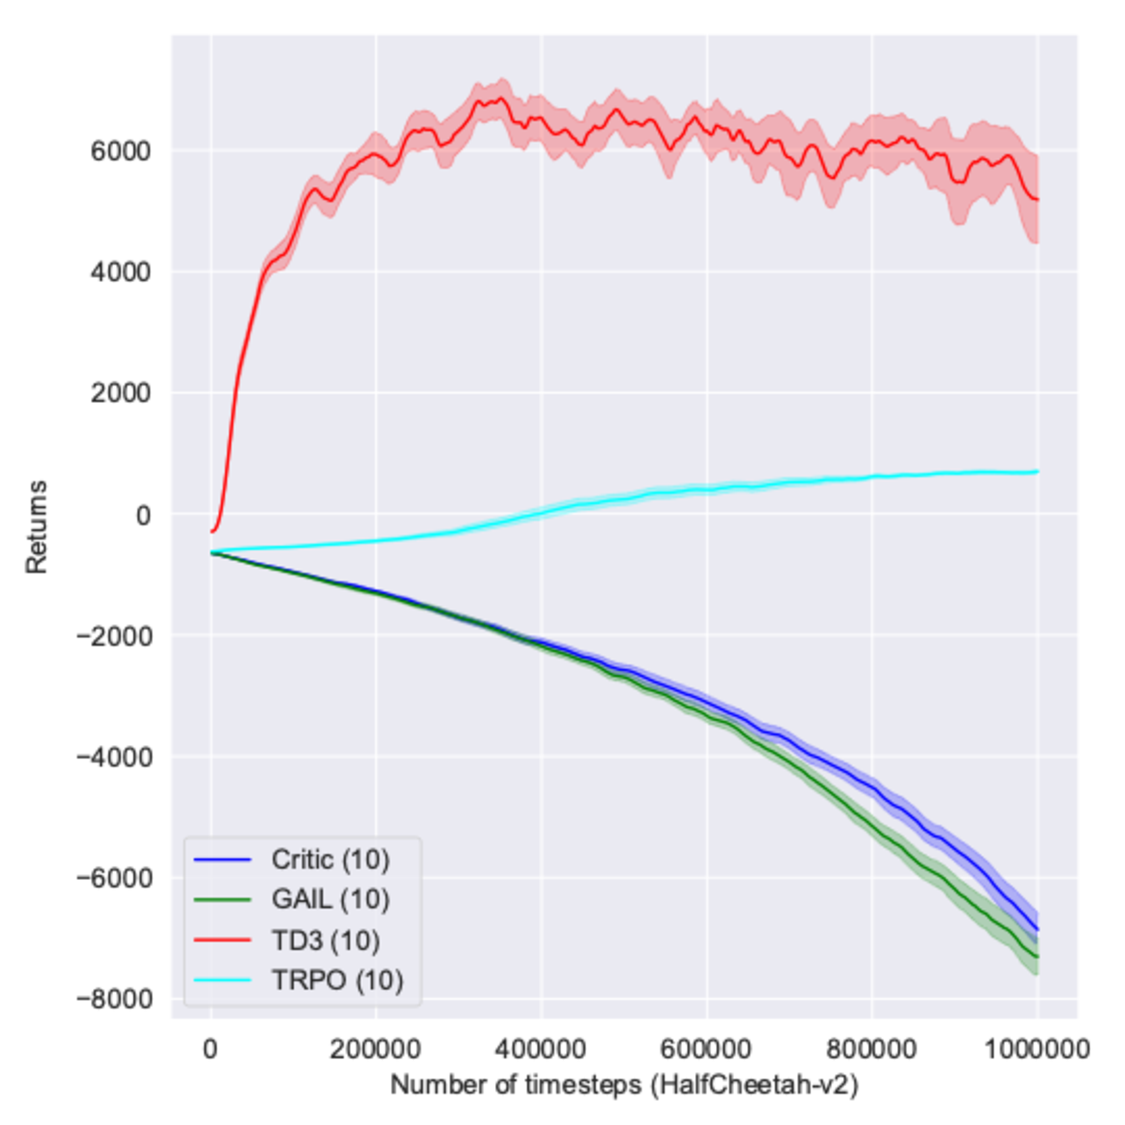
\includegraphics[width=.7\linewidth]{figures/HalfCheetah.pdf}
    \caption{Caption}
\end{figure}

\begin{figure}
    \centering
    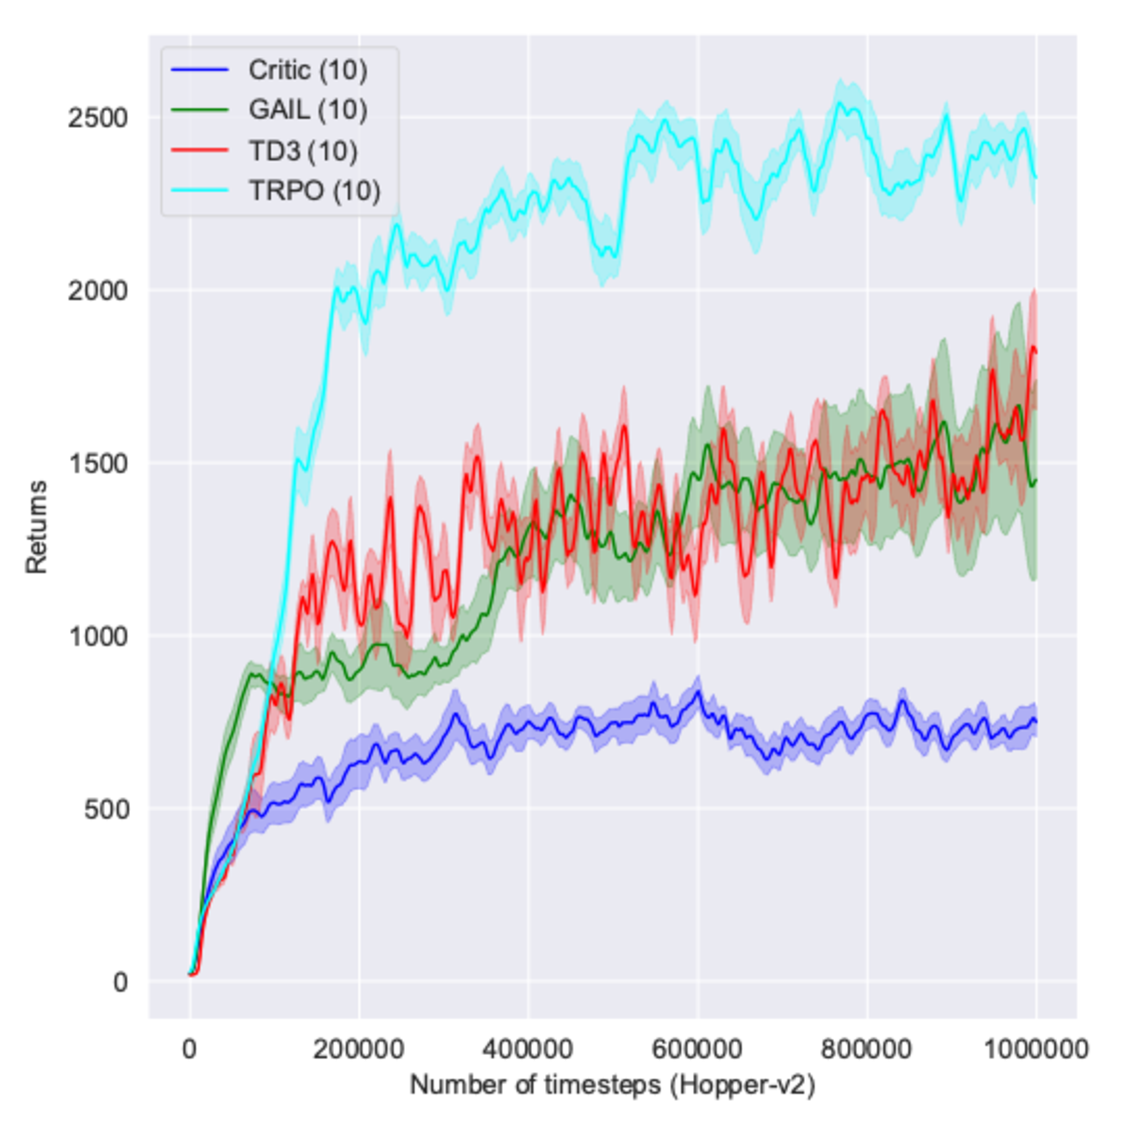
\includegraphics[width=.7\linewidth]{figures/Hopper.pdf}
    \caption{Caption}
\end{figure}

\begin{figure}
    \centering
    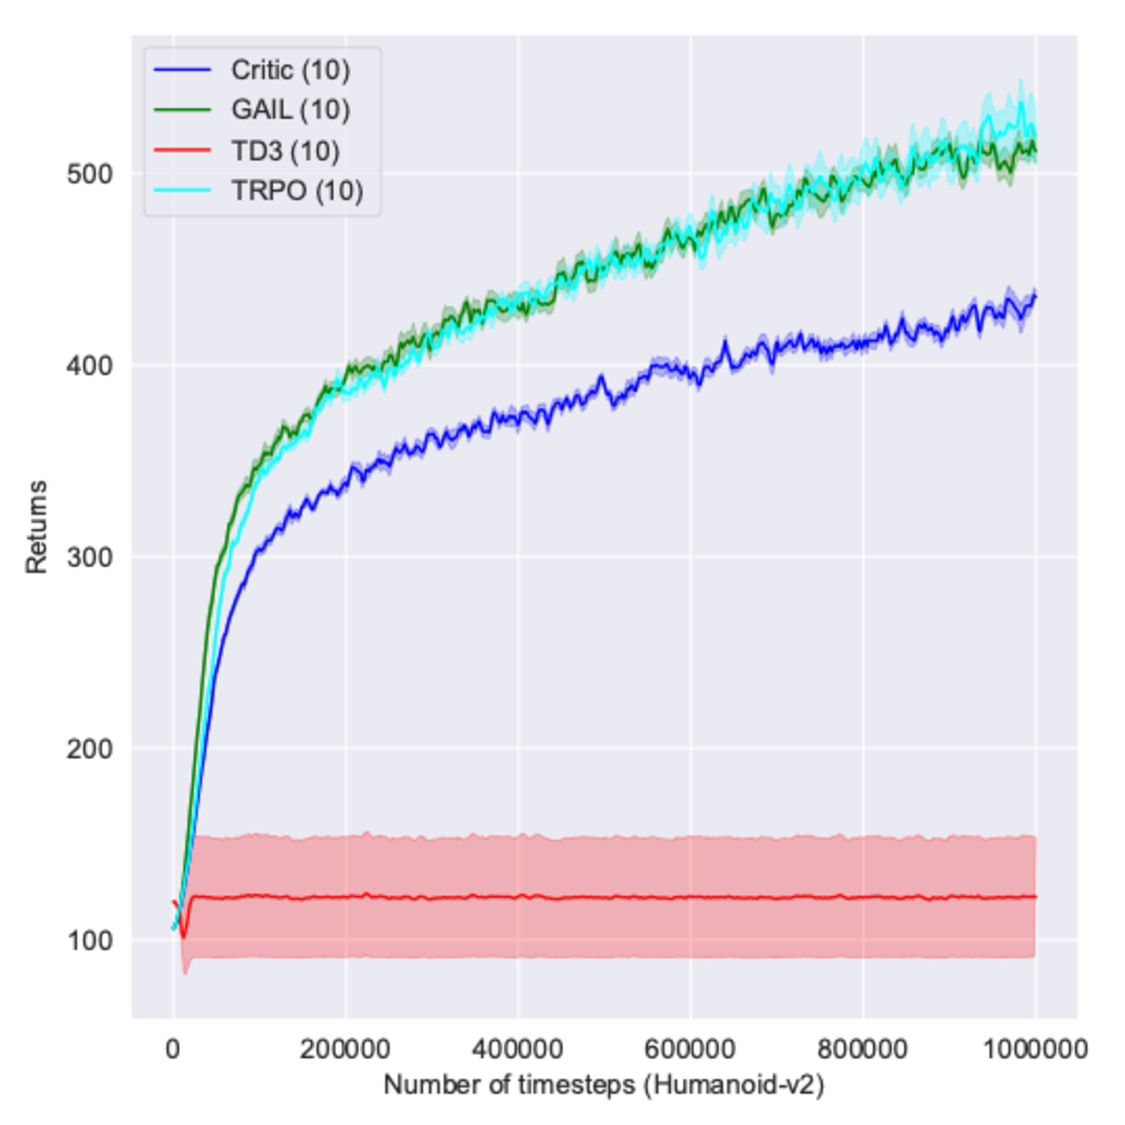
\includegraphics[width=.7\linewidth]{figures/Humanoid.pdf}
    \caption{Caption}
\end{figure}

\begin{figure}
    \centering
    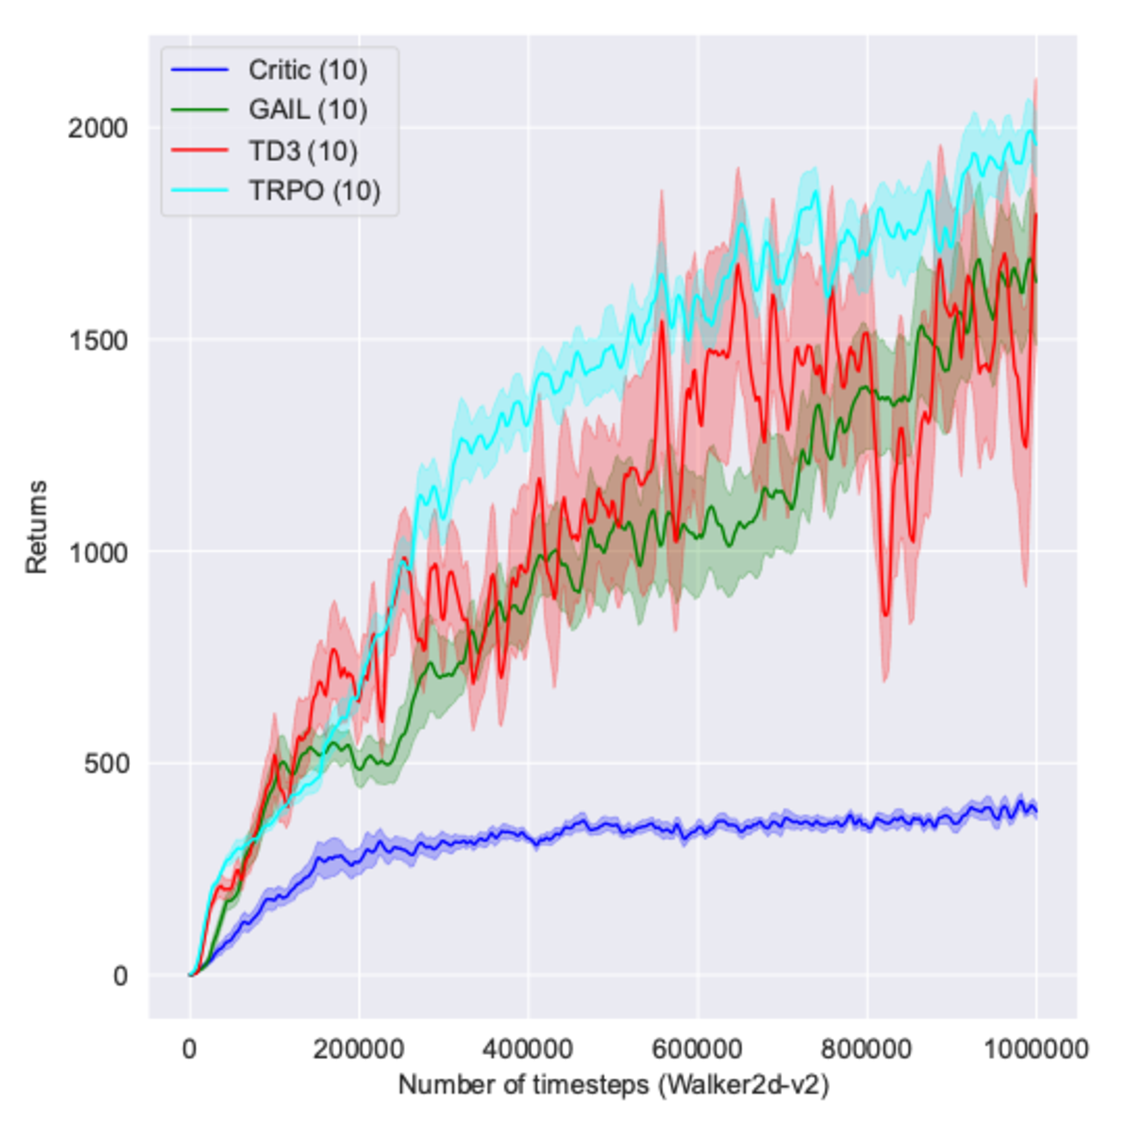
\includegraphics[width=.7\linewidth]{figures/Walker2d.pdf}
    \caption{Caption}
\end{figure}
\section{Related work}
Distribution matching approaches 

% In recent years, the development of Adversarial Imitation Learning has been mostly focused on on-policy algorithms. 
% After~\citet{ho2016generative} proposed GAIL to perform imitation learning via adversarial training, a number of extensions has been introduced. 
% Many of these applications of the AIL framework~\citep{li2017infogail,hausman2017multi,sun2019adversarial} maintain the same form of distribution estimation as GAIL which necessitates on-policy samples. 


% The connections between RL and divergence minimization have long been studied in the rich prior literature of control as probabilistic inference~\citep{todorov2007linearly,toussaint2009robot,peters2010relative,kappen2012optimal}. 
% Specifically, they have shown that optimal control under entropy regularization can be viewed as approximate inference on a graphical model, or equivalently minimizing reverse KL divergence between reward-weighted trajectory and policy trajectory distributions~\citep{kappen2012optimal,levine2018reinforcement}.
% Building on such intuitions, a number of work extended RL algorithms based on picking another divergence metric, such as forward KL~\citep{peters2007reinforcement,norouzi2016reward}, and demonstrated substantially improved empirical performances in certain situations. 
% Our work draws significant inspirations from these prior works in RL and aims to provide a probabilistic perspective in Imitation Learning (IL).
% \vit{This is a bit confusing given the title, where you say 'deterministic'.}
% \vit{gls package will free you from manually defining abbreviations. Is this the first place you define IL?}


% Similarly to RL, the connections between IRL and divergence minimization have long been alluded. 
% Early works in IRL operated by matching feature expectations or moments~\citep{abbeel2004apprenticeship} between policies and experts, a popular approach in distribution matching~\citep{dziugaite2015training,li2015generative}.
% Recent scalable approaches to Max-Ent IRL~\citep{ho2016generative}, motivated by adversarial approaches to generative modeling, demonstrate additional connections to distribution matching. 
% Concurrent to our work, \citet{ke2019imitation} also present a unifying probabilistic perspective on IL; \sw{how can it be concurrent if it was published last year?}
% however, their empirical experiments solely focus on grid world domains, while our work provides comparative results on high-dimensional continuous control environments and also evaluates the effectiveness of IL algorithms for state marginal matching~\citep{lee2019efficient}.
% \vit{Is there formulation equivalent to yours?}

\sw{It seems crucial to address the Ghasemipour paper here.}
\section{Conclusion}

\bibliography{bib}
\bibliographystyle{bib}

\appendix
\section{Appendix}
You may include other additional sections here.

\end{document}
